% Options for packages loaded elsewhere
\PassOptionsToPackage{unicode}{hyperref}
\PassOptionsToPackage{hyphens}{url}
%
\documentclass[
]{book}
\usepackage{lmodern}
\usepackage{amssymb,amsmath}
\usepackage{ifxetex,ifluatex}
\ifnum 0\ifxetex 1\fi\ifluatex 1\fi=0 % if pdftex
  \usepackage[T1]{fontenc}
  \usepackage[utf8]{inputenc}
  \usepackage{textcomp} % provide euro and other symbols
\else % if luatex or xetex
  \usepackage{unicode-math}
  \defaultfontfeatures{Scale=MatchLowercase}
  \defaultfontfeatures[\rmfamily]{Ligatures=TeX,Scale=1}
\fi
% Use upquote if available, for straight quotes in verbatim environments
\IfFileExists{upquote.sty}{\usepackage{upquote}}{}
\IfFileExists{microtype.sty}{% use microtype if available
  \usepackage[]{microtype}
  \UseMicrotypeSet[protrusion]{basicmath} % disable protrusion for tt fonts
}{}
\makeatletter
\@ifundefined{KOMAClassName}{% if non-KOMA class
  \IfFileExists{parskip.sty}{%
    \usepackage{parskip}
  }{% else
    \setlength{\parindent}{0pt}
    \setlength{\parskip}{6pt plus 2pt minus 1pt}}
}{% if KOMA class
  \KOMAoptions{parskip=half}}
\makeatother
\usepackage{xcolor}
\IfFileExists{xurl.sty}{\usepackage{xurl}}{} % add URL line breaks if available
\IfFileExists{bookmark.sty}{\usepackage{bookmark}}{\usepackage{hyperref}}
\hypersetup{
  pdftitle={CI 5371: Learning Analytics},
  pdfauthor={Bodong Chen},
  hidelinks,
  pdfcreator={LaTeX via pandoc}}
\urlstyle{same} % disable monospaced font for URLs
\usepackage{longtable,booktabs}
% Correct order of tables after \paragraph or \subparagraph
\usepackage{etoolbox}
\makeatletter
\patchcmd\longtable{\par}{\if@noskipsec\mbox{}\fi\par}{}{}
\makeatother
% Allow footnotes in longtable head/foot
\IfFileExists{footnotehyper.sty}{\usepackage{footnotehyper}}{\usepackage{footnote}}
\makesavenoteenv{longtable}
\usepackage{graphicx}
\makeatletter
\def\maxwidth{\ifdim\Gin@nat@width>\linewidth\linewidth\else\Gin@nat@width\fi}
\def\maxheight{\ifdim\Gin@nat@height>\textheight\textheight\else\Gin@nat@height\fi}
\makeatother
% Scale images if necessary, so that they will not overflow the page
% margins by default, and it is still possible to overwrite the defaults
% using explicit options in \includegraphics[width, height, ...]{}
\setkeys{Gin}{width=\maxwidth,height=\maxheight,keepaspectratio}
% Set default figure placement to htbp
\makeatletter
\def\fps@figure{htbp}
\makeatother
\setlength{\emergencystretch}{3em} % prevent overfull lines
\providecommand{\tightlist}{%
  \setlength{\itemsep}{0pt}\setlength{\parskip}{0pt}}
\setcounter{secnumdepth}{5}
\usepackage{booktabs}
\usepackage{amsthm}
\makeatletter
\def\thm@space@setup{%
  \thm@preskip=8pt plus 2pt minus 4pt
  \thm@postskip=\thm@preskip
}
\makeatother
\ifluatex
  \usepackage{selnolig}  % disable illegal ligatures
\fi
\usepackage[]{natbib}
\bibliographystyle{apalike}

\title{CI 5371: Learning Analytics}
\author{Bodong Chen}
\date{2020-12-21}

\begin{document}
\maketitle

{
\setcounter{tocdepth}{1}
\tableofcontents
}
\hypertarget{about}{%
\chapter*{About}\label{about}}
\addcontentsline{toc}{chapter}{About}

This is the course website of \textbf{CI 5371 - Learning Analytics: Theory and Practice} offered in Fall '20 at the University of Minnesota. This course is fully online. All content published on this website is \emph{open} to the public.

\textbf{Instructor}: \href{https://bodong.me/}{Bodong Chen}, Associate Professor in \href{http://www.cehd.umn.edu/ci/academics/LearningTechnologies/}{Learning Technologies} and \href{https://www.cehd.umn.edu/giving/gifts/}{Huebner Endowed Chair} in Education \& Technology.

\hypertarget{important-links}{%
\subsection*{Important Links}\label{important-links}}
\addcontentsline{toc}{subsection}{Important Links}

\begin{itemize}
\tightlist
\item
  \href{https://docs.google.com/document/d/1Y8kx_7IgM4sL9zvuG729uG6oo9p_BOxtUiNyGcDL-f8/edit?usp=sharing}{Syllabus} (public)
\item
  \href{https://la-mn.slack.com/}{Slack community} (invitation only)
\item
  \href{https://hypothes.is/}{Hypothes.is} private group (invitation only)
\item
  \href{https://twitter.com/search?q=\%23LAUMN\&src=typd}{Twitter hashtag \#LAUMN} (public)
\end{itemize}

\hypertarget{intro}{%
\chapter{Introduction}\label{intro}}

A warm welcome to \textbf{CI 5371 - Learning Analytics: Theory and Practice}! I am so excited to offer this course again this fall at the University of Minnesota. As the instructor, I learn so much from the class community each year and look forward to our adventure together this semester!

This week we will:

\begin{enumerate}
\def\labelenumi{\arabic{enumi}.}
\tightlist
\item
  Get familiar with the course, including its design, schedule, and tools
\item
  Get to know each other
\item
  Discuss our diverse interests in learning analytics
\end{enumerate}

\hypertarget{this-course}{%
\section{This Course}\label{this-course}}

\hypertarget{course-syllabus}{%
\subsection{Course Syllabus}\label{course-syllabus}}

First thing first, please read \href{https://docs.google.com/document/d/1Y8kx_7IgM4sL9zvuG729uG6oo9p_BOxtUiNyGcDL-f8/edit?usp=sharing}{\textbf{the course syllabus}} in its entirety.

Leave a comment or send me an email when you have any questions.

\hypertarget{technology-setup}{%
\subsection{Technology setup}\label{technology-setup}}

An online course does not need to be about watching videos and answering quizzes. To foster rich learning experiences, we will be using several technological tools to foster social, collaborative learning. Depending on your familiarity with these tools, there could be a learning curve. So please spend time this week to familiarize yourself with them.

\emph{Pro tip}: Please use you UMN id (\texttt{chenbd} for myself) consistently when signing up for these tools.

\textbf{Zoom}. We will host a number of virtual meetings on Zoom throughout the semester. Please make sure your computer has \href{https://zoom.us/}{Zoom} installed (see the video below). Please test your Zoom setup in advance to make sure audio and video configurations work properly.

\textbf{Slack}. You will receive a link that invites you to join \href{https://la-mn.slack.com/}{our Slack community}. Course announcements are made on Slack. All sorts of class discussions will take place there as well. You can also interact with our course alumni in some public channels. Slack is a better tool for social interaction and community building.

First time using Slack? Watch the video below and/or read this \href{https://get.slack.help/hc/en-us/articles/115004071768-What-is-Slack-}{brief introduction to Slack}.

\textbf{Hypothes.is}. You should have received a link that invites you to join our Hypothes.is group. Hypothes.is is a web annotation tool that enables us to discuss readings in a contextual manner. When annotating, please make sure our group name (\textbf{LAUMN-2020}) is properly selected (see image below). See \href{https://web.hypothes.is/help/quick-start-guide/}{this quick start guide} to get started, and \href{https://web.hypothes.is/help/annotating-with-groups/}{this tutorial page} to learn about annotating together as a group.

Again, please use your UMN id when creating your Slack and Hypothesi.is account.

\includegraphics{https://d242fdlp0qlcia.cloudfront.net/uploads/2018/03/21135305/scopeselector-groupname.png}

If you have any feedback on the design, I'd love to hear your thoughts.

\hypertarget{schedule}{%
\subsection{What to expect each week?}\label{schedule}}

This online class is designed to offer rich opportunities for social participation. Below is an infographic showing how a week would (typically) look like.

\begin{itemize}
\tightlist
\item
  \textbf{Our class meetings happen on Tuesdays.} The class meetings are designed for us to chat about things we've learned, gaps of understanding, future plans, etc. In some weeks we will meet in Zoom; in some other weeks, we will ``meet'' on Slack throughout Tuesday.
\item
  \textbf{A fresh week starts on Wednesdays.} Depending on your schedule, you can get started with course readings and begin to make annotations.
\item
  \textbf{By the end of Friday}, you are expected to finish reading articles assigned for the week and post your personal annotations on Hypothesis.
\item
  \textbf{By the end of Monday}, you are expected to check out what other colleagues annotated and reply to each other. You will receive an email notification when someone responds to you. It is hoped that by putting our minds together we can develop deeper understanding.
\item
  On Tuesday, we chat more on Slack or Zoom. Detailed guidelines will be posted each week.
\end{itemize}

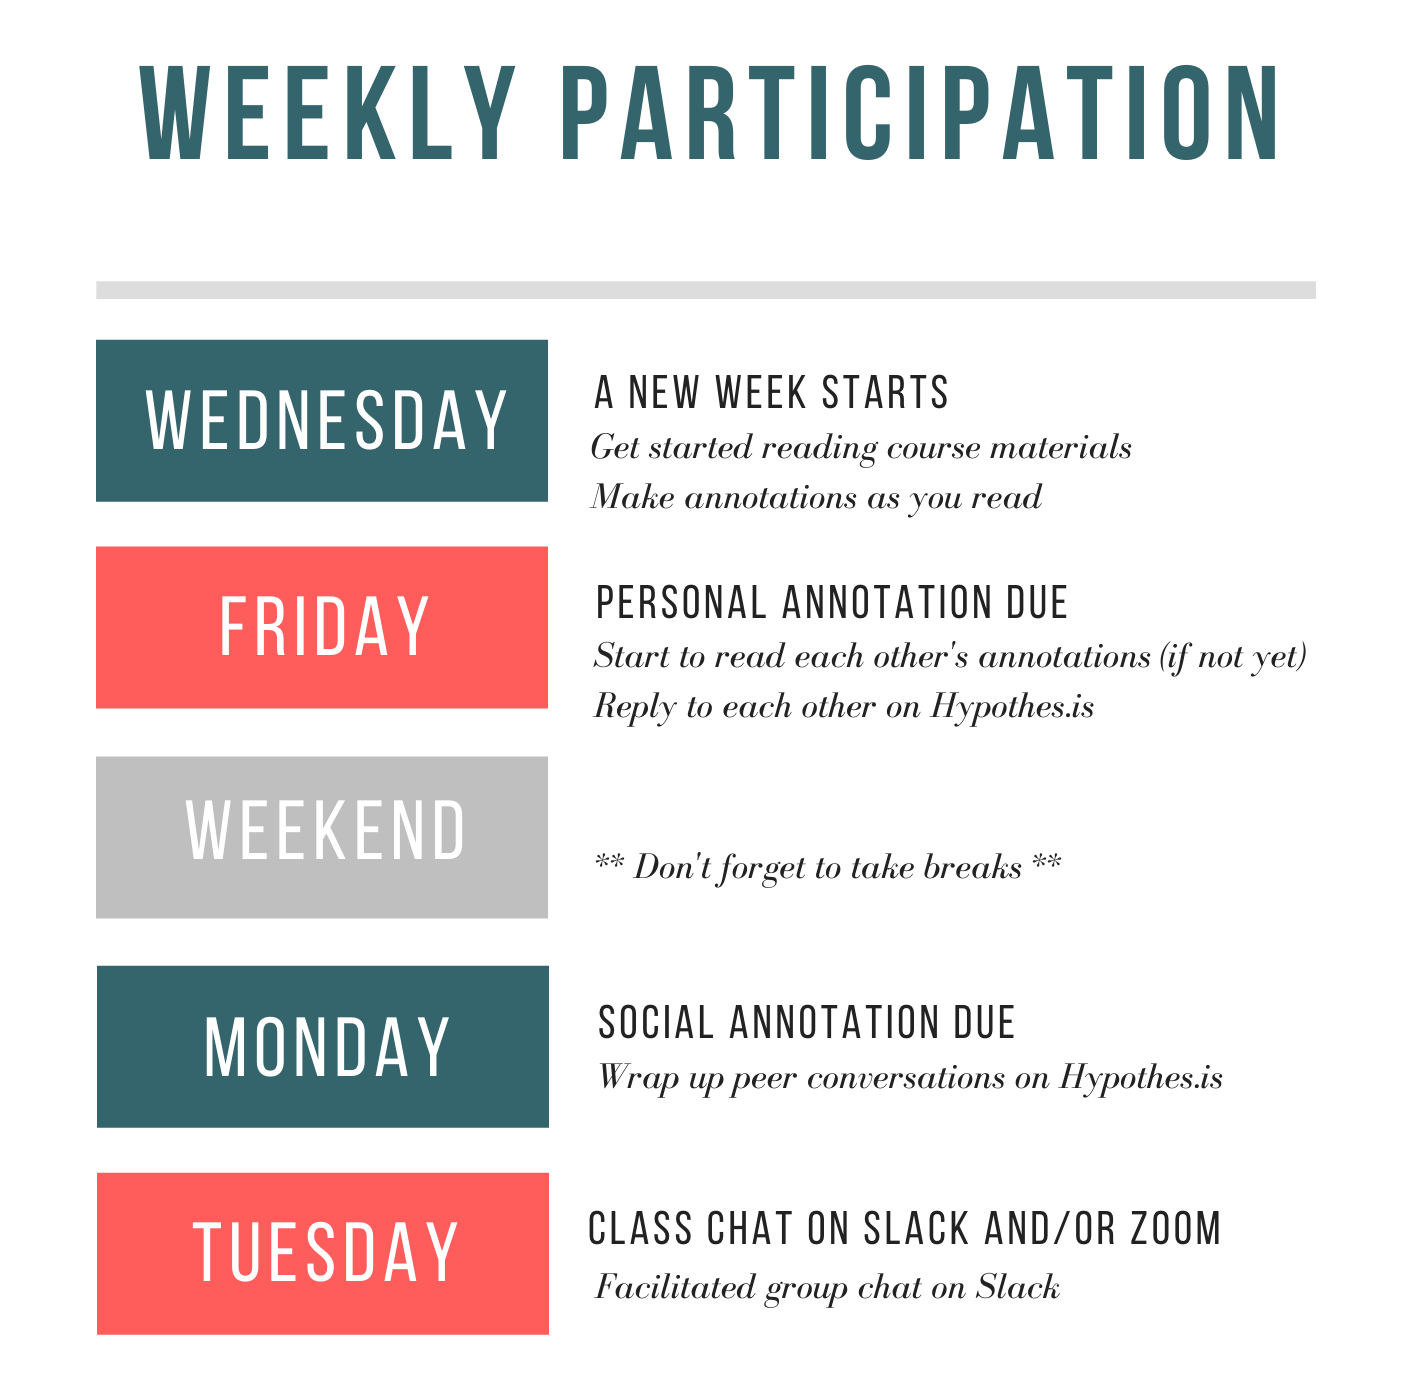
\includegraphics{img/weekly-schedule.png}

\hypertarget{week-1-activities}{%
\section{Week 1 Activities}\label{week-1-activities}}

\hypertarget{readings}{%
\subsection{Readings}\label{readings}}

\begin{enumerate}
\def\labelenumi{\arabic{enumi}.}
\tightlist
\item
  Course syllabus
\end{enumerate}

\hypertarget{week-1-zoom-meeting}{%
\subsection{Week 1 Zoom Meeting}\label{week-1-zoom-meeting}}

Our first virtual meeting will take place on \textbf{Tuesday, 09/08, 5:30-7pm} via Zoom. You should have received a calendar invitation with details.

See you soon!

\hypertarget{learning-analytics-a-brief-overview}{%
\chapter{Learning Analytics: A Brief Overview}\label{learning-analytics-a-brief-overview}}

This week we will:

\begin{enumerate}
\def\labelenumi{\arabic{enumi}.}
\tightlist
\item
  Develop a grasp of the field of LA
\item
  Start to explore course project ideas
\end{enumerate}

\hypertarget{learning-activities}{%
\section{Learning Activities}\label{learning-activities}}

\hypertarget{read-annotate-and-discuss}{%
\subsection{Read, annotate, and discuss}\label{read-annotate-and-discuss}}

This week, we will get a chance to take a closer look at this field by reading some introductory texts, exploring cases/examples, and posing questions.

\begin{itemize}
\tightlist
\item
  What problems do learning analytics seek to address?
\item
  In which educational settings?
\item
  At which levels of an education system?
\end{itemize}

Because this field is truly inter--disciplinary, I expect us to enter this field from our unique backgrounds and contribute to the field with different perspectives.

\textbf{Please read}:

\begin{enumerate}
\def\labelenumi{\arabic{enumi}.}
\tightlist
\item
  \citet{siemens2013learning} - \href{https://journals-sagepub-com.ezp2.lib.umn.edu/doi/pdf/10.1177/0002764213498851}{download link} or \href{http://journals.sagepub.com/doi/pdf/10.1177/0002764213498851}{this link}
\item
  \citet{krumm2018learning} - \textbf{\href{https://drive.google.com/open?id=1LB5J1UytIV2yOq47xKFrnneTJ7YCMJQV}{Chapter 2}} (\emph{Note: This reading can only be annotated offline. Check \href{https://www.youtube.com/watch?v=YZW6L-0qkwI}{this Youtube video} to learn how.})
\end{enumerate}

When reading each article, \textbf{please annotate} wherever you like. Let the community know when something confuses you, when you find an example that fits your interests, when you find a statement illuminating/useful, etc.

\textbf{Please also reply} to each other whenever you could. See Section \ref{schedule} posted in Week 1 for details about the weekly timeline.

This week, I encourage you to be very \textbf{intentional about tags} you use in Hypothesis annotations. Several ground rules I'd like to propose to our collective tagging to help us better index our ideas:

\begin{itemize}
\tightlist
\item
  Let's include \texttt{\#} in our tags (e.g., \texttt{\#question})
\item
  Let's use lowercase (e.g., \texttt{\#sharing}), unless the tag is a named entity (e.g., \texttt{\#LMS})
\item
  Let's not include spaces, but use underscore (\texttt{\_}) instead (e.g., \texttt{\#data\_mining} instead of \texttt{\#data\ mining})
\item
  Let's try to use the following tags when we discover \texttt{\#muddy\_points},\texttt{\#good\_points}, and \texttt{\#useful\_points} in the readings
\end{itemize}

\textbf{Reminder}: When annotating with Hypothes.is, please make sure the \texttt{LAUMN-2020} group is selected. If you are not sure about annotating PDFs, please refer back to tutorials in Week 1.

\hypertarget{watch-a-video}{%
\subsection{Watch a Video}\label{watch-a-video}}

\href{https://en.wikipedia.org/wiki/George_Siemens}{George Siemens}, who authored the first article we read, gave a lecture about learning analytics. George is the founding president of the \href{https://solaresearch.org/}{Society for Learning Analytics Research (SoLAR)}, which is the most prominent international organization of learning analytics.

Watch Siemens' lecture and share your ideas on Slack.

\hypertarget{exploring-course-project-ideas}{%
\subsection{Exploring course project ideas}\label{exploring-course-project-ideas}}

While/after reading, start to explore possible project ideas based on your interests. At this point, it is totally okay if your project idea is more or less vague. You can share your ideas on Slack. This is an opportunity for us to learn more about our interests, receive feedback, and find colleagues with similar interests.

\textbf{Below are a list of example project ideas.} Please see the syllabus for more detailed guidelines.

\begin{itemize}
\tightlist
\item
  Applying Natural Language Processing to Investigating Language Development and Epistemic Complexity in Group Chats
\item
  Integrating a Teacher Dashboard in Science Classrooms: A Mixed-Methods Study of Teacher Perspectives
\item
  Developing a Deep Learning Model for the Prediction of Student Success in Introductory Physics
\item
  Students under lockdown: Comparisons of students' social networks and mental health before and during the COVID-19 crisis
\end{itemize}

\hypertarget{week-2-zoom-meeting}{%
\subsection{Week 2 Zoom Meeting}\label{week-2-zoom-meeting}}

We will meet synchronously again on \textbf{Tuesday, 09/15, 5:30-7pm} via Zoom.

Have a great week!

\hypertarget{ethics-algorithmic-accountability-and-system-integrity}{%
\chapter{Ethics, Algorithmic Accountability, and System Integrity}\label{ethics-algorithmic-accountability-and-system-integrity}}

This week we will:

\begin{enumerate}
\def\labelenumi{\arabic{enumi}.}
\tightlist
\item
  Develop an understanding of ethics in the context of LA
\item
  Develop an awareness of theories, tools, and approaches that promote system integrity of learning analytics
\item
  Continue to explore course project ideas
\end{enumerate}

Thanks for the engaged conversations in the first week of \#LAUMN!

What is apparent to myself is that the breadth of expertise represented in our community is truly energizing. I hope we can continue to have deep conversations within and beyond this community, and to engage in learning that's personally meaningful to everyone of us.

In the spirit of ``living and exploring the capacity of learning analytics'', I encourage you to explore tools like \href{https://crowdlaaers.org/}{\textbf{CROWD LAAERS}} that we discussed during our Zoom meeting. After authenticating yourself using your \href{https://hypothes.is/account/developer}{Hypothes.is API token}, you will be able to choose our group and have a bird-eye view of our annotation activities.

I found the \texttt{Threads} section quite useful for discovering threads with more (or less) participation. You can click on a particular thread to filter or ``drill down'' the data.

\includegraphics{img/crowdlaaers-2020.png}

\hypertarget{ethics-in-learning-analytics}{%
\section{Ethics in Learning Analytics}\label{ethics-in-learning-analytics}}

Let's be clear, \emph{ethics} should not be an after-thought in a learning analytics application. (That's why we are discussing ethics this week instead of in Week 14 of this semester.) But what do ethical practices in the field entail is not always clear.

While research ethics considers principles such as confidentiality, privacy, and informed consent, a learning analytics project may not be considered \emph{research} at all (if its goal is not to produce generalizable knowledge).

However, extensive collection of learning data, increasing cases of ``black-box algorithms,'' and more direct impact on learners necessitate some serious conversations about ethics in learning analytics.

\begin{figure}
\centering
\includegraphics{https://upload.wikimedia.org/wikipedia/commons/7/7c/Blackbox3D-withGraphs.png}
\caption{(Photo Credit: \href{https://en.wikipedia.org/wiki/Black_box}{Wikipedia})}
\end{figure}

Last week's discussions have already touched upon many questions about ethics. This week, we are going to dive into ethics, algorithmic accountability, and system integrity.

\hypertarget{week-3-learning-activities}{%
\section{Week 3 Learning Activities}\label{week-3-learning-activities}}

\hypertarget{read-annotate-and-discuss}{%
\subsection{Read, annotate, and discuss}\label{read-annotate-and-discuss}}

\textbf{Please read}:

\begin{itemize}
\tightlist
\item
  \citet{prinsloo2017ethics} - \href{https://solaresearch.org/wp-content/uploads/2017/05/chapter4.pdf}{link}. (Note: It may be difficult to highlight larger text snippets in this particular PDF file.)
\item
  \textbf{Optional readings}:

  \begin{itemize}
  \tightlist
  \item
    \citet{kitto2019practical} - \href{http://sjgknight.com/finding-knowledge/wp-content/uploads/2019/08/EthicalLA-accepted_oro.pdf}{link}
  \item
    \citet{chen2019valuesensitive} - \href{https://arxiv.org/pdf/1812.08335.pdf}{link}.
  \end{itemize}
\end{itemize}

When reading each article, \textbf{please annotate} wherever you like. Let the community know when something confuses you, when you find an example that fits your interests, when you find a statement illuminating/useful, etc.

\textbf{Please also reply} to each other whenever you could. See Section \ref{schedule} posted in Week 1 for details about the weekly timeline.

This week, I encourage you to be very \textbf{intentional about tags} you use in Hypothesis annotations.

\textbf{Reminder}: When annotating with Hypothes.is, please make sure the \texttt{LAUMN-2020} group is selected. If you are not sure about annotating PDFs, please refer back to this video tutorial.

\hypertarget{meet-learning-analytics-experts}{%
\subsection{Meet Learning Analytics Experts}\label{meet-learning-analytics-experts}}

\textbf{\href{https://opendistanceteachingandlearning.wordpress.com/about/}{Paul Prinsloo}} from the University of South Africa (Unisa) has been writing and giving talks about `ethics and learning analytics' for many years. He delivered a keynote on this topic in Scotland in 2018. He has graciously allowed me to embed his slides on our course website:

Zombie categories, broken data and biased algorithms: What else can go wrong? Ethics in the collection, analysis and use of student data from University of South Africa (Unisa)

\textbf{\href{http://simon.buckinghamshum.net/}{Simon Buckingham Shum}}, Director of the Connected Intelligence Centre (CIC) at the University of Technology Sydney, invited us to consider `Algorithmic Accountability' and `Analytic System Integrity'. Discussion of Algorithmic Accountability has been \href{https://www.acm.org/binaries/content/assets/public-policy/2017_usacm_statement_algorithms.pdf}{taken up by important academic associations like the Association for Computing Machinery (ACM)}. But Simon stretches our thinking to consider `Analytic System Integrity' in learning analytics. Below is a talk he gave at the UCL Institute of Education in 2016. His team is recently working on \href{http://simon.buckinghamshum.net/2018/08/ethical-design-critique/}{Ethical Design Critique}, which offers concrete measures to enhance ethics in learning analytics tools. And he is delivering a Learning Informatics Webinar to a UMN audience on Sep 24! Don't miss it.

\hypertarget{living-with-learning-analytics}{%
\subsection{``Living'' with Learning Analytics}\label{living-with-learning-analytics}}

Last week, we introduced \href{https://crowdlaaers.org/}{CROWD LAAERS} designed for Hypothes.is.

This week, I encourage you to check out \href{https://jonudell.info/h/facet/}{\textbf{this data tool}} developed by a Hypothes.is engineer that helps you ``see'' Hypothes.is data. Again, you will need to use your Hypothes.is API token to access our private group annotations. Please try to play with the CSV and JSON formats to see what they look like.

Share your thoughts and findings on Slack!

\hypertarget{continuing-to-explore-project-ideas}{%
\subsection{Continuing to explore project ideas}\label{continuing-to-explore-project-ideas}}

Thanks for sharing your initial project ideas on Slack. As we read and discuss more, please take time to explore and refine ideas. The official deadline for sharing your project idea is 9/29.

Please consider \emph{problems/goals}, \emph{stakeholders}, \emph{data sources}, \emph{analysis}, and \emph{action} of your project.

When you're ready, please post your project idea in the \texttt{projects} channel. Continue to give each other's ideas constructive comments!

\includegraphics{https://media.giphy.com/media/13HBDT4QSTpveU/giphy.gif}

\hypertarget{housekeeping}{%
\section{Housekeeping}\label{housekeeping}}

\hypertarget{start-to-explore-special-interest-groups-sigs}{%
\subsection{Start to Explore Special Interest Groups (SIGs)}\label{start-to-explore-special-interest-groups-sigs}}

\textbf{Please start to consider which Special Interest Group(s) you're interested in.} Below is a list of tentative topics but you can suggest topics beyond the list. Ideally, the Special Interest Group you sign up for is related to your final project.

\begin{itemize}
\tightlist
\item
  Social Network Analysis
\item
  Predictive Models
\item
  Text and Discourse Analytics
\item
  Visual Learning Analytics
\item
  Temporal Analytics
\item
  Multimodal Learning Analytics
\item
  Collaboration Analytics
\item
  Institutional Readiness
\end{itemize}

\hypertarget{future-weeks}{%
\subsection{Future Weeks}\label{future-weeks}}

No Zoom meetings in the next few weeks.

There will be a Slack chat on Tue, Sep 22 (details to be announced).

Questions? Reach out to Bodong via Slack or email.

\hypertarget{cases-and-examples-of-learning-analytics}{%
\chapter{Cases and Examples of Learning Analytics}\label{cases-and-examples-of-learning-analytics}}

This week we will:

\begin{enumerate}
\def\labelenumi{\arabic{enumi}.}
\tightlist
\item
  Develop familiarity with ways computational methods can be used to support research
\item
  Develop familiarity with real-world learning analytics tools and applications
\item
  Continue to explore course project ideas
\end{enumerate}

Thanks for the engaged conversations on both Hypothes.is and Slack! Great collaborative work (like \href{https://hyp.is/NFor1vhTEeq9wSM8TXN_OQ/www.solaresearch.org/wp-content/uploads/2017/05/chapter4.pdf}{this thread}) as we make sense of complex ideas in course readings. Please keep it up!

Two Pro Tips about Hypothes.is:

\begin{enumerate}
\def\labelenumi{\arabic{enumi}.}
\tightlist
\item
  If you prefer to not see existing highlights when reading an article, click on the Hide/Show Highlights button on the sidebar.\\
  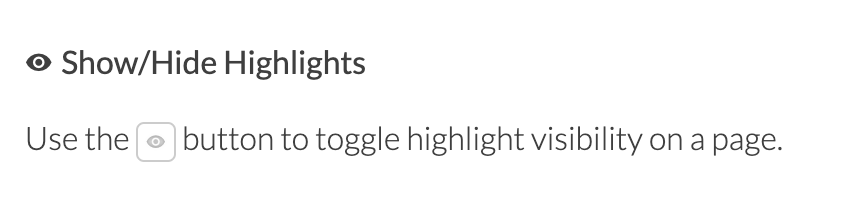
\includegraphics{img/h_hide_highlights.png}
\item
  You can also resize the sidebar, click and hold on the Arrow button and then drag to resize the sidebar.\\
  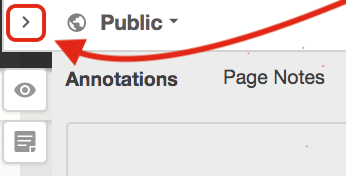
\includegraphics{img/h-resize-sidebar.png}
\end{enumerate}

\hypertarget{learning-analytics-cases-and-examples}{%
\section{Learning Analytics Cases and Examples}\label{learning-analytics-cases-and-examples}}

After reading and discussing several key articles about learning analytics, I hope it is becoming clearer that there are often two types of work involved when people talk about learning analytics:

\begin{enumerate}
\def\labelenumi{\arabic{enumi}.}
\tightlist
\item
  \textbf{Applying computational methods} (or data science methods) to learning data to help us understand complex learning phenomena
\item
  \textbf{Designing and deploying tools} that are based on computational analysis of learning data to make an impact in a learning context
\end{enumerate}

Researchers of learning (e.g.~learning scientists) may feel more drawn to the first, while folks who engineer tools or work closely with people who make day-to-day decisions in education (e.g.~teachers, advisers, students, administrators) could be more attracted to the latter. Of course, these two lines are not clear-cut but deeply intertwined.

Both lines require us to think carefully about ethics, accountability, and integrity in the work, even though the considerations and coping strategies may differ between these two lines.

\hypertarget{week-4-learning-activities}{%
\section{Week 4 Learning Activities}\label{week-4-learning-activities}}

This week, we will explore and analyze more concrete cases/examples of learning analytics.

Following the distinction made above, you can purposefully target one type of work in your interest area.

Use Hypothes.is as a social annotation tool for example. As a researcher, I am curious about what factors are driving our social interaction and would be interested in learning data science methods that would allow me to model social interaction. As a learning technologist, I am also interested in supporting instructors who teach online classes using Hypothes.is. What information might be useful for their decision-making? How to best present such information? And, to tell you the truth, I am actually interested in both directions!

Please take time to think about your interests at this moment so that your exploration can become more targetted.

\hypertarget{meet-two-experts}{%
\subsection{Meet Two Experts}\label{meet-two-experts}}

Before we dive into identifying and analyzing cases, I want to share two talks that are related to this week and the projects you are working on.

The first talk was given by \textbf{\href{https://www.si.umich.edu/people/stephanie-teasley}{Dr.~Stephanie Teasley}} from the University of Michigan, a powerhouse of learning analytics research \& practice. Teasley is a past president of SoLAR and has been leading various learning analytics efforts at UMich, including the \textbf{\emph{My Learning Analytics (MyLA)}} project that is piloted at UMN. She gave a talk, titled ``\textbf{Learning Analytics: Data Science for Education}'', which covers many grounds including analytics tool design and evaluation.

The second talk was given by \textbf{\href{http://roberto.martinezmaldonado.net/}{Dr.~Roberto Martinez-Maldonado}} from Monash University, who previously worked at the Connected Intelligence Centre (CIC) of the University of Technology Sydney. This talk is about a a \emph{Multimodal Learning Analytics} project in a medical education setting. You can find more details in \href{https://dl.acm.org/doi/abs/10.1145/3313831.3376148}{their paper here} published in the hyper-competitive CHI conference.

\hypertarget{case-analysis}{%
\subsection{Case analysis}\label{case-analysis}}

After watching these videos, please conduct a learning analytics \emph{case analysis} following these two main steps.

\hypertarget{a-identify}{%
\subsubsection*{(a) Identify}\label{a-identify}}
\addcontentsline{toc}{subsubsection}{(a) Identify}

Ideally, you will \textbf{identify minimally one case/example} potentially relevant to your project idea.

I am providing only a few examples below but you should absolutely go beyond this list.

\begin{itemize}
\tightlist
\item
  Course Signals: \href{https://er.educause.edu/articles/2010/3/signals-applying-academic-analytics}{EDUCAUSE article}, \href{https://www.youtube.com/watch?v=kURsmrkdS04}{LAK12 video}
\item
  ECoach: \url{https://ecoach.ai.umich.edu/Welcome/}
\item
  Academic Writing Analytics: \url{https://utscic.edu.au/tools/awa/}
\item
  My Learning Analytics (MyLA): \url{https://sites.google.com/umich.edu/my-learning-analytics-help/home}
\item
  Yellowdig visualization tool: \url{https://vimeo.com/169580885}
\end{itemize}

\hypertarget{b-analyze-and-share}{%
\subsubsection*{(b) Analyze and Share}\label{b-analyze-and-share}}
\addcontentsline{toc}{subsubsection}{(b) Analyze and Share}

When analyzing a case/example, please consider the following aspects:

\begin{longtable}[]{@{}ll@{}}
\toprule
\emph{Aspects of the project} & \emph{Your analysis}\tabularnewline
\midrule
\endhead
Name and links &\tabularnewline
Context and stakeholders &\tabularnewline
Project goals &\tabularnewline
Learning constructs &\tabularnewline
Data sources &\tabularnewline
Data analysis/mining techniques &\tabularnewline
Actions suggested or taken &\tabularnewline
Ethical considerations &\tabularnewline
\bottomrule
\end{longtable}

To share your analysis with the class, please post a Slack message in the \texttt{2020-general} channel with these components.

To allow us to learn from each other's work, \textbf{please share your case analysis by the end of Sep 28.}

\hypertarget{project-ideas-share-out}{%
\subsection{Project ideas share-out}\label{project-ideas-share-out}}

Hope the case analysis is helpful for your exploration of project ideas.

When you're ready, please craft a blurb about your initial project idea and post it in the \#projects channel. Please consider \emph{problems/goals}, \emph{stakeholders}, \emph{data sources}, \emph{analysis}, and \emph{action} of your group project. \textbf{Please post by the end of Sep 29.}

\hypertarget{housekeeping}{%
\section{Housekeeping}\label{housekeeping}}

\hypertarget{continue-to-explore-special-interest-groups-sigs}{%
\subsection{Continue to Explore Special Interest Groups (SIGs)}\label{continue-to-explore-special-interest-groups-sigs}}

Please continue to consider which Special Interest Group(s) you're interested in. Below is a list of tentative topics but you can suggest topics beyond the list. Ideally, the Special Interest Group you sign up for is related to your final project. I will distribute a signup page next week.

\begin{itemize}
\tightlist
\item
  Social Network Analysis
\item
  Predictive Models
\item
  Text and Discourse Analytics
\item
  Visual Learning Analytics
\item
  Temporal Analytics
\item
  Multimodal Learning Analytics
\item
  Collaboration Analytics
\item
  Institutional Readiness
\end{itemize}

\hypertarget{future-weeks}{%
\subsection{Future Weeks}\label{future-weeks}}

No Zoom meetings in the next few weeks.

Questions? Reach out to Bodong via Slack or email.

\hypertarget{theory-and-learning-analytics}{%
\chapter{Theory and Learning Analytics}\label{theory-and-learning-analytics}}

\href{https://link.springer.com/article/10.1007\%2Fs11528-014-0822-x}{Learning analytics are about learning}, so \emph{theories of learning} should not be ditched despite the data deluge that has been fueling the growth of learning analytics.

Since the dawn of the field, there have been voices arguing for the importance of learning theory in the design, development, and implementation of learning analytics. In 2015, \href{https://learning-analytics.info/journals/index.php/JLA/issue/view/358}{a special section} was published by the \emph{Journal of Learning Analytics} on the relation between learning theory and learning analytics. In the guest editorial, Wise and Shaffer (2015, p.~5) write:

\begin{quote}
It is an exhilarating and important time for conducting research on learning, with unprecedented quantities of data available. There is danger, however, in thinking that with enough data, the numbers speak for themselves. In fact, with larger amounts of data, theory plays an ever-more critical role in analysis.
\end{quote}

The notion that theory matters even more in ``big data'' research in education goes against what was proposed in a controversial \emph{Wired} article titled ``\href{https://www.wired.com/2008/06/pb-theory/}{The end of theory: The data deluge makes the scientific method obsolete}'' (Anderson, 2008). Now there is little disagreement that learning theory is essential for learning analytics.

\hypertarget{learning-analytics-and-learning-theory}{%
\section{Learning Analytics and Learning Theory}\label{learning-analytics-and-learning-theory}}

Briefly speaking, there are essentially two ways theory is important for the field of learning analytics.

\textbf{1. Theory Use in Learning Analytics}

As a field of research and practice, learning analytics work naturally draws from all sorts of theories. As summarized by Wise and Shaffer (2015, p.~9):

\begin{itemize}
\tightlist
\item
  Theory gives a researcher guidance about which variables to include in a model
\item
  Theory gives a researcher guidance about what potential confounds, subgroups, or covariates in the data to account for
\item
  Theory gives a researcher guidance as to which results to attend to
\item
  Theory gives a researcher a framework for interpreting results
\item
  Theory gives a researcher guidance about how to make results actionable
\item
  Theory helps a researcher generalize results to other contexts and populations
\end{itemize}

For example, \emph{self-regulated learning} (SRL) is widely used in learning analytics and MOOC research. SRL as a learning theory has informed data collection, data transformation, data mining, and result interpretation.

\textbf{2. Theory Building in Learning Analytics}

Even more exciting to me is the possibility of building new theories of learning and teaching, based on fine-grained data analysis enabled by advanced computational methods. Learning analytics and educational data mining research could give rise to new theories. For example, whether keystroke analysis can shed light on our understanding of writing processes? Whether temporal analysis can uncover ``productive'' patterns of collaborative discourse?

Equally valuable are theories of learning analytics usage in emerging socio-technical contexts. For example, as new learning analytics tools are put in the hands of instructors to aid their pedagogical decisions, domain theories of analytics use can be created (e.g., van Leeuwen, 2015).

After exploring cases and proposing possible project ideas last week, it is a great time for us to think about learning theory relevant to our project ideas!

\hypertarget{week-5-learning-activities}{%
\section{Week 5 Learning Activities}\label{week-5-learning-activities}}

\hypertarget{read-annotate-and-discuss}{%
\subsection{Read, annotate, and discuss}\label{read-annotate-and-discuss}}

This week's readings speak in particular to \emph{theory use} in learning analytics. \textbf{Reading \#2} provides a concrete example of using a well-established learning theory (self-regulated learning in this case) in a research study. \textbf{Reading \#3} (optional) is the controversial Wired article mentioned above.

\begin{enumerate}
\def\labelenumi{\arabic{enumi}.}
\tightlist
\item
  \textbf{Skim}: \citet{wise2015why} - \href{https://files.eric.ed.gov/fulltext/EJ1127063.pdf}{download link}. This reading is a guest editorial about learning analytics and learning theory. Please skim through it and no need to annotate closely.
\item
  \textbf{Read \& Annotate}: \citet{winne2017learning} - \href{https://solaresearch.org/wp-content/uploads/2017/05/chapter21.pdf}{download link}. This reading discusses a very established learning theory -- Self-Regulated Learning (SRL) -- that is widely adopted in learning analytics. Please read and take time to ``notice'' how the author discusses SRL and connects SRL constructs with data.
\item
  \textbf{Skim}: \citet{kizilcec2017selfregulated} - \href{https://www-sciencedirect-com.ezp3.lib.umn.edu/science/article/pii/S0360131516301798}{download link} (\emph{Note: This file is accessible via the UMN Libraries.}) The third reading is a study that examines SRL in MOOCs. Please skim through it to see how the authors used SRL theory to grapple with the learning phenomenon.
\end{enumerate}

As always, please annotate and interact as you like. Please use tags intentionally in your annotations to help you retrieve ideas potentially useful for our course projects.

As a reminder, please strive to stick to the weekly participation schedule:
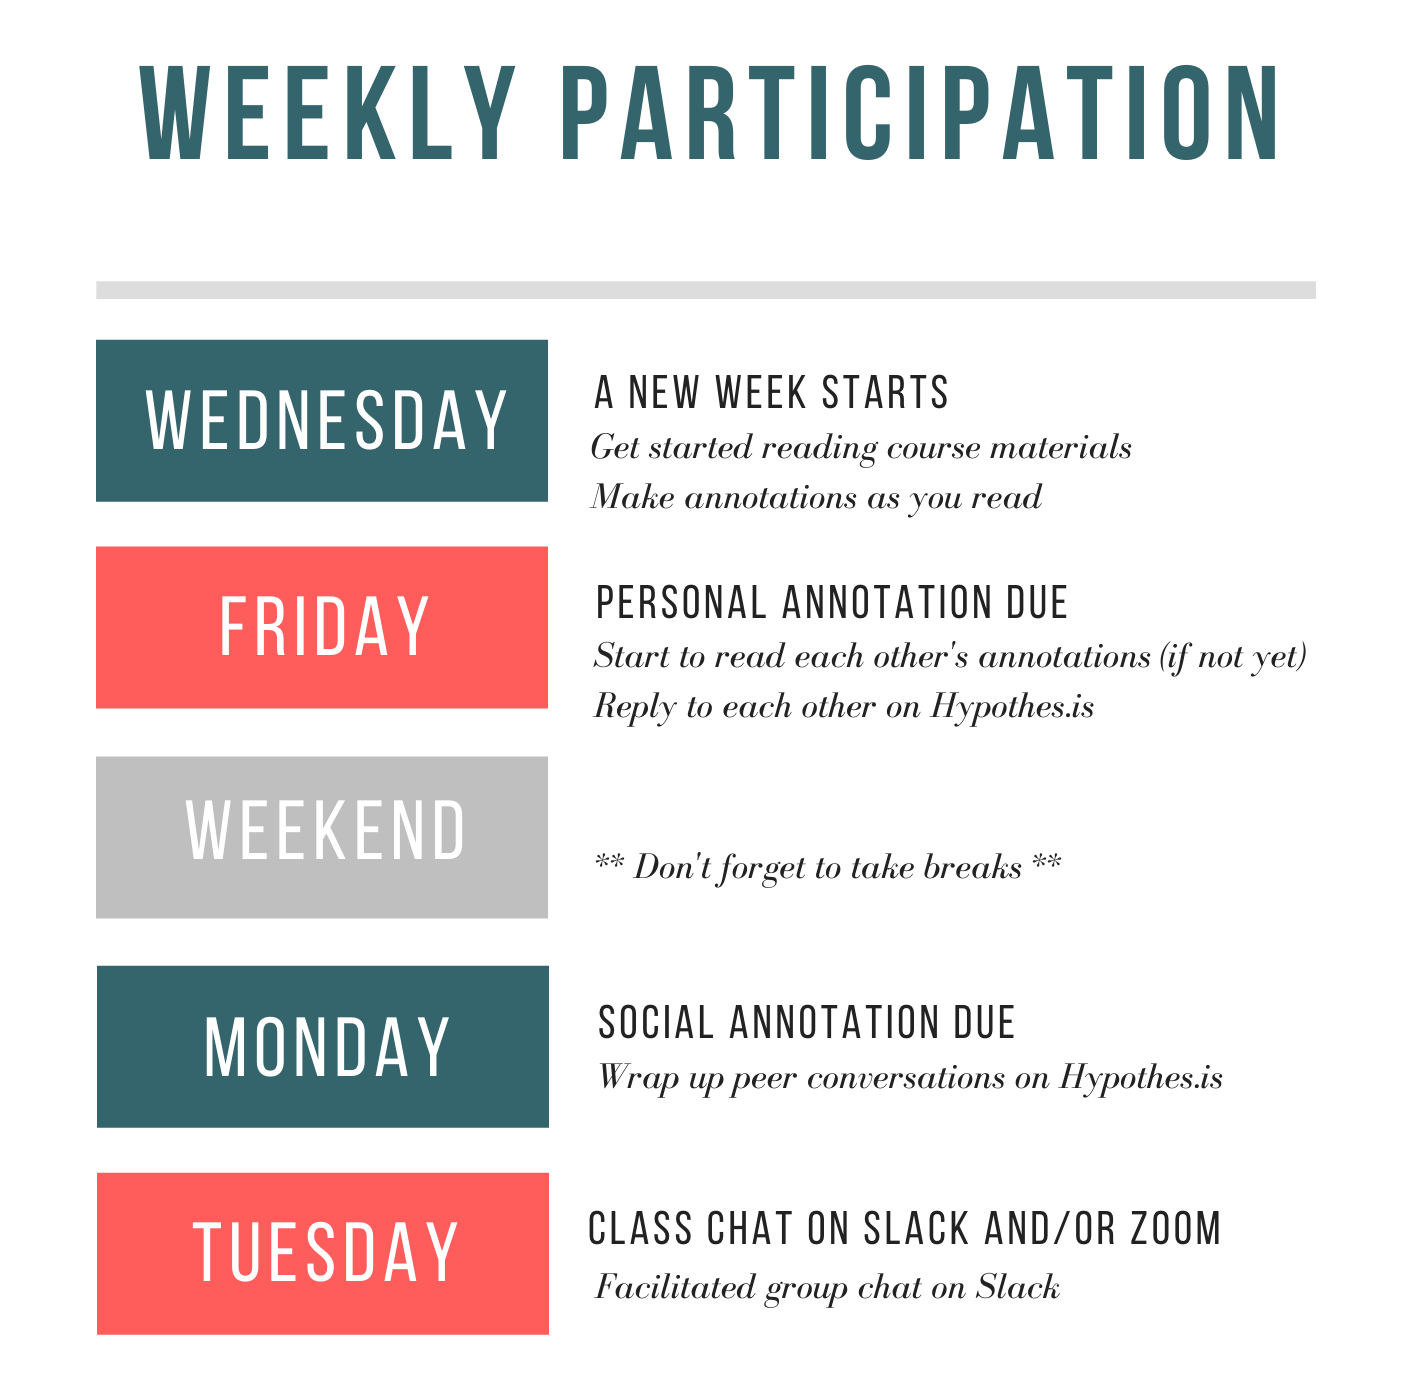
\includegraphics{img/weekly-schedule.png}

\hypertarget{meet-learning-analytics-experts}{%
\subsection{Meet Learning Analytics Experts}\label{meet-learning-analytics-experts}}

\textbf{\href{https://edpsych.education.wisc.edu/staff/williamson-shaffer-david/}{Dr.~David Williamson Shaffer}} is the Vilas Distinguished Professor of Learning Sciences at the University of Wisconsin-Madison. He is known for his work on game-based learning and \href{http://www.epistemicanalytics.org/}{Epistemic Network Analysis}. Below is a keynote speech he delivered at the 2018 Learning Analytics and Knowledge conference in Sydney, where he summarized his idea of ``quantitative ethonography'' and ways to tackle theory scarcity in the age of ``big data.''

\hypertarget{special-interest-group-sig-signup}{%
\subsection{Special Interest Group (SIG) Signup}\label{special-interest-group-sig-signup}}

I will distribute a SIG signup form on Slack. Please fill the form with your preferred topics.

As a reminder:

\begin{quote}
``With support from the instructor, each SIG is expected to take a lead on designing learning activities, presenting key ideas, and facilitating discussion. Each SIG will meet with the instructor one week in advance to finalize their course plan.'' (From course syllabus)
\end{quote}

Feel free to ask questions on Slack if you're unsure about any SIG topics.

\hypertarget{continue-to-advance-your-project-idea}{%
\subsection{Continue to advance your project idea}\label{continue-to-advance-your-project-idea}}

Please continue to articulate or advance your project idea. Use this week's readings and discussions to help you more clearly conceptualize the learning phenomenon you're interested in. Do some literature search to find out theories relevant to your project. Share in the \texttt{\#projects} channel things you find!

Have a great week!

\includegraphics{https://images.pexels.com/photos/64775/pexels-photo-64775.jpeg?auto=compress\&cs=tinysrgb\&dpr=2\&h=750\&w=1260}

\hypertarget{hidden-assumptions-epistemology-pedagogy-and-assessment}{%
\chapter{Hidden Assumptions: Epistemology, Pedagogy, and Assessment}\label{hidden-assumptions-epistemology-pedagogy-and-assessment}}

In this week, we will extend our dialogues on \emph{learning theory} in the previous week into deeper conversations about hidden assumptions in learning analytics.

This line of thinking has been informed by a talk given by \textbf{\href{https://twitter.com/sjgknight?lang=en}{Simon Knight}} at LAK13 titled \emph{Epistemology, Pedagogy, Assessment and Learning Analytic} (see slides below). Their work has evolved over the years and one reading for this week is a book chapter with a set of provocations pushing us to think more about hidden assumptions.

LAK13: Epistemology, Pedagogy, Assessment and Learning Analytics from Simon Knight

I've \href{https://www.researchgate.net/publication/317586037_Unpacking_Learning_Analytics_An_Attempt_to_Tilt_the_Iceberg_jiexixuexifenxixueyiciqiaodongbingshandechangshi}{written about this topic as well, in my mother tongue Chinese}. To me,

\begin{quote}
``Learning Analytics is like an iceberg. Its visible parts include materialized tools and observable activities, while its hidden parts comprise conceptualizations of learning, power relations in teaching and learning, and complex social, political and cultural intentions of education.''
\end{quote}

Catering to the Chinese audience, I drew on \href{https://www.vividict.com/Public/index/page/details/details.html?rid=11671}{the etymology of the character 数 (\emph{n}: number; \emph{v}: count) in Chinese} and explained how one of its ancient forms (below) is embedded with the meaning of punishing someone (esp.~a kid) for their ``mistakes.''

\includegraphics{https://www.vividict.com/Upload/2020/1/3/20200103111043147908.png}

I could not stop asking: \emph{To what extent is this original meaning still reflected in our use of numbers or data (数据) today? Which other assumptions and biases are built into our daily data practices in general and learning analytics in particular? How about in other languages or cultures?}

\hypertarget{meet-an-expert}{%
\section{Meet An Expert}\label{meet-an-expert}}

Last week we read the book chapter by Dr.~\href{https://www.sfu.ca/education/faculty-profiles/pwinne.html}{Phil Winne}, Professor from Simon Fraser University, Canada. I recently encountered this interview he did with the Centre for Change and Complexity in Learning (C3L), University of South Australia. Take a look to find out why he joined the learning analytics community and what he thinks the biggest challenges are for the field.

\hypertarget{week-6-learning-activities}{%
\section{Week 6 Learning Activities}\label{week-6-learning-activities}}

\hypertarget{read-annotate-and-discuss}{%
\subsection{Read, annotate, and discuss}\label{read-annotate-and-discuss}}

We have two readings for this week -- one short book chapter and one journal article.

\begin{enumerate}
\def\labelenumi{\arabic{enumi}.}
\tightlist
\item
  \citet{knight2017theory} - \href{https://solaresearch.org/wp-content/uploads/2017/05/chapter1.pdf}{link}
\item
  \citet{perrotta2018social} - \href{https://www.tandfonline.com/doi/pdf/10.1080/17439884.2016.1182927?needAccess=true}{link}
\end{enumerate}

As always, please annotate and interact as you like. As I suggested last week, you can make annotations at your own pace using your preferred medium.

\begin{quote}
``I invite everyone to come up with a strategy that works for you. One example: Read through quickly and make highlights (even on paper). Then pick a few key spots to make annotations that would help yourself and others in the class.''
\end{quote}

As we work towards forming our SIGs and course projects, it would be great to think about making \emph{some of} your annotations more useful for your SIG planning and final project. I encourage you to think about useful tags, e.g., \texttt{\#SIG\_social\_network}, \texttt{\#PROJ\_dental\_course}, and then use them to purposefully tag your annotations. By doing so, we will be able to index our ideas as we continue to engage with all sorts of resources. Again, you may choose to read through an article first and come back to annotate or tag important annotations.

\hypertarget{sig-planning}{%
\subsection{SIG planning}\label{sig-planning}}

First of all, \textbf{please finalize your Special Interest Group (SIG) choices.} Feel free to ask questions on Slack.

If you have assembled a group, congratulations! As for next steps, I suggest you consider the following when launching your SIG efforts:

\begin{itemize}
\tightlist
\item
  On Slack, create a new \emph{channel} dedicated to your SIG. You don't need to invite everyone yet, but you can start to chat with your SIG co-lead. Feel free to invite Bodong in to co-plan with you.
\end{itemize}

\hypertarget{continue-to-advance-your-project-idea}{%
\subsection{Continue to advance your project idea}\label{continue-to-advance-your-project-idea}}

At this point, you can tell that I'm trying to structure each week for you to keep advancing your course project. Last week, treat your Slack post about learning theory as a step forward for your course project. The next few weeks will be similar.

Again, it is totally fine if your current project idea still feels vague. But please do seek out opportunities to advance your ideas by searching additional resources or chatting with each other via Slack. My hope is to make sure everyone in this course is building a project that has a purpose beyond this course. You are in charge of making the final project meaningful for youself!

Have a great week ahead!

\includegraphics{https://media1.tenor.com/images/9b141e57cccfc60a9f214e97b9061e69/tenor.gif?itemid=4529300}

\hypertarget{educational-data-mining-an-overview}{%
\chapter{Educational Data Mining: An Overview}\label{educational-data-mining-an-overview}}

\begin{figure}
\centering
\includegraphics{https://images.pexels.com/photos/1009928/pexels-photo-1009928.jpeg?auto=compress\&cs=tinysrgb\&dpr=2\&h=750\&w=1260}
\caption{Image credit: \href{https://www.pexels.com/photo/yellow-heavy-equipment-1009928/}{\textbf{pixabay}}}
\end{figure}

As a sister field of Learning Analytics, \textbf{Educational Data Mining (EDM)} emerged a few years earlier and has its own disciplinary identity (e.g., a stonger computer science focus, its own \href{http://educationaldatamining.org/about/}{professional society}, \href{http://educationaldatamining.org/conferences/}{conference}, and \href{https://jedm.educationaldatamining.org/index.php/JEDM}{journal}). While two communities developed separately in the beginning, \href{http://www.upenn.edu/learninganalytics/ryanbaker/LAKs\%20reformatting\%20v2.pdf}{communication and collaboration between two communities (PDF)} have increased over the years.

The overlaps and differences between two communities are nicely summarized by \href{http://journals.sagepub.com/doi/10.1177/0002764213498851}{Siemens (2013)}:

\begin{quote}
Where LA is more concerned with sensemaking and action, educational data mining (EDM) is more focused toward developing methods for ``exploring the unique types of data that come from educational settings''. Although the techniques used are similar in both fields, EDM has a more specific focus on reductionist analysis (Siemens \& Baker, 2012). As LA draws from and extends EDM methodologies (Bienkowski, Feng, \& Means, 2012, p.~14), it is a reasonable expectation that the future development of analytic techniques and tools from both communities will overlap.
\end{quote}

We are diving into EDM this week by exploring its connections with LA and playing with various data mining tools used in both communities.

\includegraphics{http://educationaldatamining.org/EDM_ORG/wp-content/uploads/2017/09/edm.png}

\hypertarget{meet-an-expert}{%
\section{Meet an Expert}\label{meet-an-expert}}

\textbf{Candace Thille} is the founding director of the Open Learning Initiative (OLI) at Carnegie Mellon University and at Stanford University. Her focus is in applying the results from research in the science of learning to the design and evaluation of open web-based learning environments and in using those environments to conduct research in human learning. She took a leave from Stanford \href{https://www.insidehighered.com/digital-learning/article/2018/01/29/amazons-high-profile-hire-higher-education-candace-thille}{in 2018 to work for Amazon}. In this talk she gave in 2016, she explored the intersection among the science of learning, data, analytics, and technologies.

\hypertarget{week-7-learning-activities}{%
\section{Week 7 Learning Activities}\label{week-7-learning-activities}}

\hypertarget{read-annotate-and-discuss}{%
\subsection{Read, annotate, and discuss}\label{read-annotate-and-discuss}}

We have two readings this week -- one presenting an overview and the other introducing many useful tools.

\begin{enumerate}
\def\labelenumi{\arabic{enumi}.}
\tightlist
\item
  \citet{romero2020educational} - \href{files/Romero\%20and\%20Ventura\%20-\%202020.pdf}{PDF link}
\item
  \citet{slater2017tools} - \href{files/Slater\%20et\%20al.\%20-\%202017.pdf}{PDF link}
\end{enumerate}

As always, please annotate and interact as you like.

As we work towards forming our SIGs and course projects, it would be great to think about making \emph{some of} your annotations more useful for your SIG planning and final project. I encourage you to think about useful tags, e.g., \texttt{\#SIG\_social\_network}, \texttt{\#PROJ\_dental\_course}, and then use them to purposefully tag your annotations. By doing so, we will be able to index our ideas as we continue to engage with all sorts of resources. Again, you may choose to read through an article first and come back to annotate or tag important annotations.

Note: These tags need to used accurately (e.g.~spaces and caps matter) in order to be nicely aggregated by Hypothes.is.

\hypertarget{sig-planning}{%
\subsection{SIG Planning}\label{sig-planning}}

Since we've finalized \textbf{our Special Interest Group plan}, please create channels on Slack, invite group members in, and get the planning started.

\hypertarget{register-for-the-next-learning-informatics-webinar}{%
\subsection{Register for the next Learning Informatics Webinar}\label{register-for-the-next-learning-informatics-webinar}}

I strongly encourage you to attend the next \textbf{Learning Informatics Seminar on Oct 27}, featuring Dr.~Marcelo Worsley. \href{https://umn.zoom.us/webinar/register/WN_S6aW-qPcQDS-v-XihTNf_A}{RSVP here}!

Let the party begin!

\includegraphics{https://thumbs.gfycat.com/WeakAnyBallpython-size_restricted.gif}

\hypertarget{bonus-video-how-to-easily-export-hypothes.is-annotations}{%
\section{Bonus video: How to easily export Hypothes.is annotations?}\label{bonus-video-how-to-easily-export-hypothes.is-annotations}}

Since some of you expressed an interest in using Hypothes.is in your own research, I made this short video to demonstrate my workflow. Let me know if you have any clarification questions.

\hypertarget{all-about-data-data-wrangling}{%
\chapter{`All About Data,' Data Wrangling"}\label{all-about-data-data-wrangling}}

\begin{figure}
\centering
\includegraphics{https://images.pexels.com/photos/1251179/pexels-photo-1251179.jpeg?auto=compress\&cs=tinysrgb\&dpr=2\&h=750\&w=1260}
\caption{Image credit: \href{https://www.pexels.com/photo/person-flattening-dough-with-rolling-pin-1251179/}{\textbf{pixabay}}}
\end{figure}

\textbf{Data wrangling}, or data munging, is a critical part of any learning analytics project. It covers multiple components of the \emph{Learning Analytics Model} including the collection, storage, cleaning, and integration of data (see Siemens 2013, which we read in \href{_book/learning-analytics-a-brief-overview.html}{Week 2}).

\begin{figure}
\centering
\includegraphics{https://c1.staticflickr.com/3/2814/9662456144_51b12d6057_b.jpg}
\caption{LA Model by Siemens}
\end{figure}

Due to the quantity of data and the diversity of data sources, a learning analytics project often necessicitates data wrangling -- conducted by humans -- in order to transform data into actionable intelligence and systematic action (\href{https://dl.acm.org/citation.cfm?doid=2567574.2567603}{Clow, 2012}).

This week, we will:

\begin{enumerate}
\def\labelenumi{\arabic{enumi}.}
\tightlist
\item
  Familiarzie with the concept of data wrangling
\item
  Play with at least one data-wrangling tool of your choice
\item
  Share your data-wranglinge experiences with peers
\item
  Draft a data-wrangling plan for your course project
\end{enumerate}

\hypertarget{what-is-data-wrangling}{%
\section{What is data wrangling?}\label{what-is-data-wrangling}}

According to \href{https://en.wikipedia.org/wiki/Data_wrangling}{Wikipedia}:

\begin{quote}
\textbf{Data wrangling}, sometimes referred to as data munging, is the process of transforming and mapping data from one ``raw'' data form into another format with the intent of making it more appropriate and valuable for a variety of downstream purposes such as analytics. A \textbf{data wrangler} is a person who performs these transformation operations.
\end{quote}

Over the past years, I have seen polls of data scientists (like \href{https://www.forbes.com/sites/gilpress/2016/03/23/data-preparation-most-time-consuming-least-enjoyable-data-science-task-survey-says/\#4d660d346f63}{this one}) showing they spend 60\% of their time `massaging' instead of analyzing data. This percentage may even go up to 80-90\% \href{https://www.infoworld.com/article/3228245/data-science/the-80-20-data-science-dilemma.html}{in some reports}.

``90\% of data science is wrangling data, the other 10\% is complaining about wrangling data.''\citet{evelgab} at \#rstatsnyc

--- David Robinson (\citet{drob}) April 20, 2018

\hypertarget{week-8-learning-activities}{%
\section{Week 8 Learning Activities}\label{week-8-learning-activities}}

As your course projects continue to take shape, this week provides us an opportunity to \textbf{consider the data aspect} and \textbf{draft a Data Wrangling plan} for your project.

Below are activities designed for this week.

\hypertarget{watch-a-lecture-on-data-wrangling}{%
\subsection*{1. Watch a lecture on data wrangling}\label{watch-a-lecture-on-data-wrangling}}
\addcontentsline{toc}{subsection}{1. Watch a lecture on data wrangling}

This lecture was delivered by \href{https://blog.ouseful.info/about/}{\textbf{Tony Hirst}} to the \href{https://www.edx.org/course/data-analytics-learning-utarlingtonx-link5-10x}{\emph{Data, Analytics and Learning} MOOC} in 2014. (This video is still one of the best I could find on this topic desipte its `age'.) Tony is an active blogger, and \href{https://blog.ouseful.info/}{his blog} has always been a great source of inspiration for me.

If you're an R user, I also recommend this talk given by \href{https://ch.linkedin.com/in/stianhaklev}{\textbf{Stian Håklev}}, Sr.~Engineer and Learning Architect at Minerva Project. He demonstrated almost a complete workflow going from messy, dirty Coursera data to some nice visualizations.

\hypertarget{play-with-one-data-wranging-tool-of-your-choice}{%
\subsection*{2. Play with one data wranging tool of your choice}\label{play-with-one-data-wranging-tool-of-your-choice}}
\addcontentsline{toc}{subsection}{2. Play with one data wranging tool of your choice}

Our choices include -- but are not limited to -- the following:

\textbf{Spreadsheets}. Yes, spreadsheets (e.g.~Excel, Google Sheets) are incredibly powerful when it comes to data wrangling. Below are two tutorials that may help you unleash the power of spreadsheets.

\begin{itemize}
\tightlist
\item
  \href{https://schoolofdata.org/courses/\#IntroDataCleaning}{School of Data: A Gentle Introduction to Data Cleaning}
\item
  \href{http://www.datacarpentry.org/spreadsheet-ecology-lesson/}{Data Carpentry: Data Organization in Spreadsheets}
\end{itemize}

\textbf{OpenRefine}, formerly Google Refine, ``is a powerful tool for working with messy data: cleaning it; transforming it from one format into another; and extending it with web services and external data.'' \href{http://openrefine.org/}{Its official website} provides several introductory videos to get you started. There is \href{https://datacarpentry.org/openrefine-socialsci/}{a Data Capentry course on OpenRefine for Social Science Data}.

\textbf{Trifacta Wrangler}. This tool was created by a Stanford/Berkeley group and then lead to a company named Trifacta. Wrangler is an interactive tool for data cleaning. It takes messy, real-world data and transforms it into data tables. Then you can export to Excel, Tableau, R, etc. See \href{https://www.trifacta.com/data-wrangling/}{this link} for details.

\textbf{R and RStudio}. If you know R basics, I strongly encourage you to spend some time on the \texttt{tidyverse} ecosystem. It has absolutely transformed my data wrangling practices in R.

\begin{itemize}
\tightlist
\item
  \href{https://www.rstudio.com/resources/webinars/data-wrangling-with-r-and-rstudio/}{RStudio webinar on data wrangling}
\item
  \href{https://www.lynda.com/R-tutorials/Data-Wrangling-R/594442-2.html}{Lynda.com course on Data wrangling with R and RStudio}
\end{itemize}

\textbf{Python}, another popular programming language among data scientists. There are plenty of tutorioals out there. Below are just two examples.

\begin{itemize}
\tightlist
\item
  \href{https://towardsdatascience.com/wrangling-data-with-pandas-27ef828aff01}{Wrangling data with \texttt{Pandas}}
\item
  \href{https://medium.com/ibm-watson-data-lab/wrangle-data-in-jupyter-notebooks-with-pixiedust-rosie-7d9ac1129925}{Wrangle Data in Jupyter Notebooks with \texttt{PixieDust\ Rosie}}
\end{itemize}

This list is by no means exhaustive or comprehensive. \textbf{Is there a data wrangling tool you like? Please share on Slack.}

Not sure what data to use? \textbf{Please consider exporting your Hypothes.is annotation data with the \href{https://jonudell.info/h/facet/}{Facet tool}.}

Finally, check out the \href{https://datacarpentry.org/lessons/\#social-science-curriculum}{Data Carpentry} website that offers a range of lessons and workshops that you may find useful.

\hypertarget{share-your-journey-as-a-data-wrangler-via-slack}{%
\subsection*{3. Share your journey as a Data Wrangler via Slack}\label{share-your-journey-as-a-data-wrangler-via-slack}}
\addcontentsline{toc}{subsection}{3. Share your journey as a Data Wrangler via Slack}

\includegraphics{https://upload.wikimedia.org/wikipedia/en/thumb/f/ff/SuccessKid.jpg/256px-SuccessKid.jpg}

Yes, we can do it! How did your journey go? Have you discovered your data-wrangling superpower? Share a blurb about your journey in the \texttt{\#2020-general} channel of Slack. If you choose to blog your experience, please post a link to your blog post to the \texttt{\#2020-general} Slack channel.

If you encounter data wrangling challenges, please also feel free to share on Slack so that we can problem solve together.

\hypertarget{craft-a-data-wrangling-plan-for-your-course-project}{%
\subsection*{4. Craft a data-wrangling plan for your course project}\label{craft-a-data-wrangling-plan-for-your-course-project}}
\addcontentsline{toc}{subsection}{4. Craft a data-wrangling plan for your course project}

What implications does this week's work have on your course project? You will be asked to share out your data-wrangling ideas on Tuesday via Slack.

\hypertarget{housekeeping-for-formal-participation}{%
\section{Housekeeping for Formal Participation}\label{housekeeping-for-formal-participation}}

To all SIGs, please start planning your SIG activities.

Our first SIG meeting is scheduled to happen on 11/3. Given it's the election day, we may need to shift the plan. Stay tuned.

Enjoy digging and wrangling!

\includegraphics{http://gif-finder.com/wp-content/uploads/2016/06/Dog-Digging.gif}

  \bibliography{book.bib,packages.bib}

\end{document}
